\documentclass[11pt,a4paper]{article}
\usepackage[utf8]{inputenc}
\usepackage[T1]{fontenc}
\usepackage[english]{babel}
\usepackage{tabularx}
\usepackage[a4paper,margin=1.5cm]{geometry}

\usepackage{amsmath, amssymb}

\usepackage{graphicx}
\usepackage{float}

\usepackage{booktabs}
\usepackage{caption}
\usepackage{subcaption}

\usepackage{listings}
\usepackage{xcolor}
\usepackage{siunitx} % for aligned numeric columns
\sisetup{round-mode=places, round-precision=2}

\usepackage{pgfplots}
\usepackage{polyglossia}


\pgfplotsset{compat=1.18}
\usepackage{pgfplotstable}

\usepackage[hidelinks]{hyperref}

\title{Sorting Algorithm Benchmark Report}
\author{Michał Łasocha}
\date{\today}

\begin{document}

\maketitle
\tableofcontents
\newpage

\section{Introduction}
This report will go over presentation, implementation and benchmarking of
multiple sorting algorithm, using go programming language.
\section{Selected algorithms}
I have selected 7 different algorithms for the purpose of this report:
\begin{itemize}

	\item \textbf{Bubble Sort}
	      \begin{itemize}
		      \item \textit{Design}: Simple comparison-based algorithm that repeatedly swaps adjacent elements if they are out of order, "bubbling" the largest element to the end on each pass.
		      \item \textit{Implementation}: Self-implemented
		      \item \textit{Best Case Complexity}: \(O(n)\) — when the array is already sorted (with optimization).
		      \item \textit{Worst Case Complexity}: \(O(n^2)\) — when the array is sorted in reverse.
	      \end{itemize}

	\item \textbf{Bucket Sort}
	      \begin{itemize}
		      \item \textit{Design}: Distributes elements into buckets, sorts each bucket (usually with another algorithm), then concatenates the buckets. Works best with uniformly distributed data.
		      \item \textit{Best Case Complexity}: \(O(n + k)\) — with \(k\) buckets and evenly distributed data.
		      \item \textit{Implementation}: Self-implemented
		      \item \textit{Worst Case Complexity}: \(O(n^2)\) — if all elements fall into one bucket.
	      \end{itemize}

	\item \textbf{Go's Built-in Sort (sort.Ints)}
	      \begin{itemize}
		      \item \textit{Design}: Hybrid adaptive sort (introsort) combining quicksort, heapsort, and insertion sort based on input.
		      \item \textit{Implementation}: Go standard library
		      \item \textit{Best Case Complexity}: \(O(n \log n)\)
		      \item \textit{Worst Case Complexity}: \(O(n \log n)\) — guaranteed by switching to heapsort if needed.
	      \end{itemize}

	\item \textbf{Heap Sort}
	      \begin{itemize}
		      \item \textit{Design}: Builds a max-heap and repeatedly extracts the maximum element, maintaining the heap property.
		      \item \textit{Implementation}: Self-implemented
		      \item \textit{Best Case Complexity}: \(O(n \log n)\)
		      \item \textit{Worst Case Complexity}: \(O(n \log n)\)
	      \end{itemize}

	\item \textbf{Insertion Sort}
	      \begin{itemize}
		      \item \textit{Design}: Builds the sorted array by inserting each element into its correct position.
		      \item \textit{Implementation}: Self-implemented
		      \item \textit{Best Case Complexity}: \(O(n)\) — when the array is already sorted.
		      \item \textit{Worst Case Complexity}: \(O(n^2)\) — when the array is reverse sorted.
	      \end{itemize}

	\item \textbf{QuickSort}
	      \begin{itemize}
		      \item \textit{Design}: Divide-and-conquer algorithm selecting a pivot, partitioning the array, then recursively sorting subarrays.
		      \item \textit{Implementation}: Self-implemented
		      \item \textit{Best Case Complexity}: \(O(n \log n)\) — balanced partitions.
		      \item \textit{Worst Case Complexity}: \(O(n^2)\) — consistently unbalanced partitions.
	      \end{itemize}

	\item \textbf{Radix Sort (Signed)}
	      \begin{itemize}
		      \item \textit{Design}: Non-comparative integer sort processing digits from least significant to most significant, adapted for signed integers.
		      \item \textit{Implementation}: Self-implemented
		      \item \textit{Best Case Complexity}: \(O(nk)\), where \(k\) is the number of digit positions.
		      \item \textit{Worst Case Complexity}: \(O(nk)\) — depends mainly on digit count, not input order.
	      \end{itemize}

	\item \textbf{Threaded Merge Sort (Parallel Merge Sort)}
	      \begin{itemize}
		      \item \textit{Design}: Splits array into parts, sorts them in parallel threads, then merges sorted subarrays.
		      \item \textit{Implementation}: Self-implemented
		      \item \textit{Best Case Complexity}: \(O\left(\frac{n \log n}{p} + \text{overhead}\right)\), where \(p\) is number of threads.
		      \item \textit{Worst Case Complexity}: \(O\left(\frac{n \log n}{p} + \text{overhead}\right)\).
	      \end{itemize}


\end{itemize}

\section{Experimental Setup and Methodology}
Following system and hardware were used in order to obtain the data presented later in the report:
\subsection{Environment}
\begin{itemize}
	\item \textit{Hardware}: Ryzen 9 7900X (12C/24T), 32 GB DDR5 RAM
	\item \textit{Operating system}: Gnu/Linux 6.14.6-zen1-1-zen
	\item \textit{Programming Language and runtime}: go version go1.24.3 linux/amd64
\end{itemize}

\subsection{Methodology}

All Algorithms were implemented or imported in main.go package, with use of go standard library.
Self-implemented algorithms were validated using unit tests provided inside of
the main\_test.go package.

Each algorithm was written with integer sorting in mind, with minimal
non-compiler optimizations, using slices in place of arrays, and goroutines in
place of threads.

Threaded algorithms were written in mind to adapt to user's thread count and
use worker groups in order to maximal efficiency and avoid thread starting
overhead where possible.

All sorting Algorithms would be benched using the implemented BenchmarkSort and
BenchmarkSortNoReturn functions that measure time in milliseconds. Program
generates multiple differently sized arrays of random integers and runs each
algorithm while measure time over all runs, returning average time. All times
are logged into a csv file for further data processing using LibreOffice Calc.

\subsection{Early predictions}
Go's built in sort's hybrid design should deliver the best results for average
cases, while remaining competitive with massive data sets. Algorithms such as
insertion sort will perform well on small data sets, but will fail to compete
with other algorithms  with large datasets. Parallel Merge Sort will have poor
results with small data sets, due to overhead caused by its threaded design,
however it should by far scale the best with extreme size data sets due to it
being able to split the workload across multiple threads.

\newpage
\section{Results}
\subsection{Raw data}
The raw data represents the direct timing outputs from the benchmark runs,
collected over multiple iterations for each algorithm and input size. It is
stored in CSV format without filtering. Algorithms such as Insertion sort and
especially Bubble sort were skipped at 10 million  and 100 million element
arrays, as time for soting would be measured in hours, making it completely unusable.
\begin{table}[H]
	\centering
	\scriptsize
	\begin{tabularx}{\textwidth}{|r|*{8}{>{\centering\arraybackslash}X|}c|}
		\hline
		\textbf{Size}         & \textbf{Bubble Sort} & \textbf{Bucket Sort} & \textbf{Go's built-in Sort} & \textbf{Heap Sort} & \textbf{Insertion Sort} & \textbf{QuickSort} & \textbf{Radix Sort} & \textbf{Threaded Merge Sort} & \textbf{Total Result} \\
		\hline
		100                   & 3.02                 & 1.8                  & 0.01                        & 1.11               & 1.03                    & 8.87               & 1.09                & 4.48                         & 21.41                 \\
		1000                  & 487.13               & 13.68                & 7.9                         & 21.67              & 106.79                  & 165.14             & 18.98               & 40.26                        & 861.55                \\
		10000                 & 28210                & 278.61               & 353.36                      & 550.6              & 9263.46                 & 1584.91            & 182.7               & 307.7                        & 40731.34              \\
		100000                & 6180190              & 4044.6               & 4327.9                      & 7614.9             & 863296.8                & 21757.8            & 3221.3              & 4045.1                       & 7088498.4             \\
		1000000               &                      & 32787.8              & 47876                       & 96219.2            &                         & 203230.6           & 26929.6             & 18241.8                      & 425285                \\
		10000000              &                      & 551177.8             & 550829.4                    & 1650828.2          &                         & 2047687.6          & 297298              & 157711                       & 5255532               \\
		\hline
		\textbf{Total Result} & 6208890.15           & 588304.29            & 603394.57                   & 1755235.68         & 872668.08               & 2274434.92         & 327651.67           & 180350.34                    & 12810929.7            \\
		\hline
	\end{tabularx}
	\caption{Sorting algorithm benchmark times (ms) by input size.}
\end{table}

\subsection{Processed data}

\begin{figure}[H]
	\begin{center}
		\graphicspath[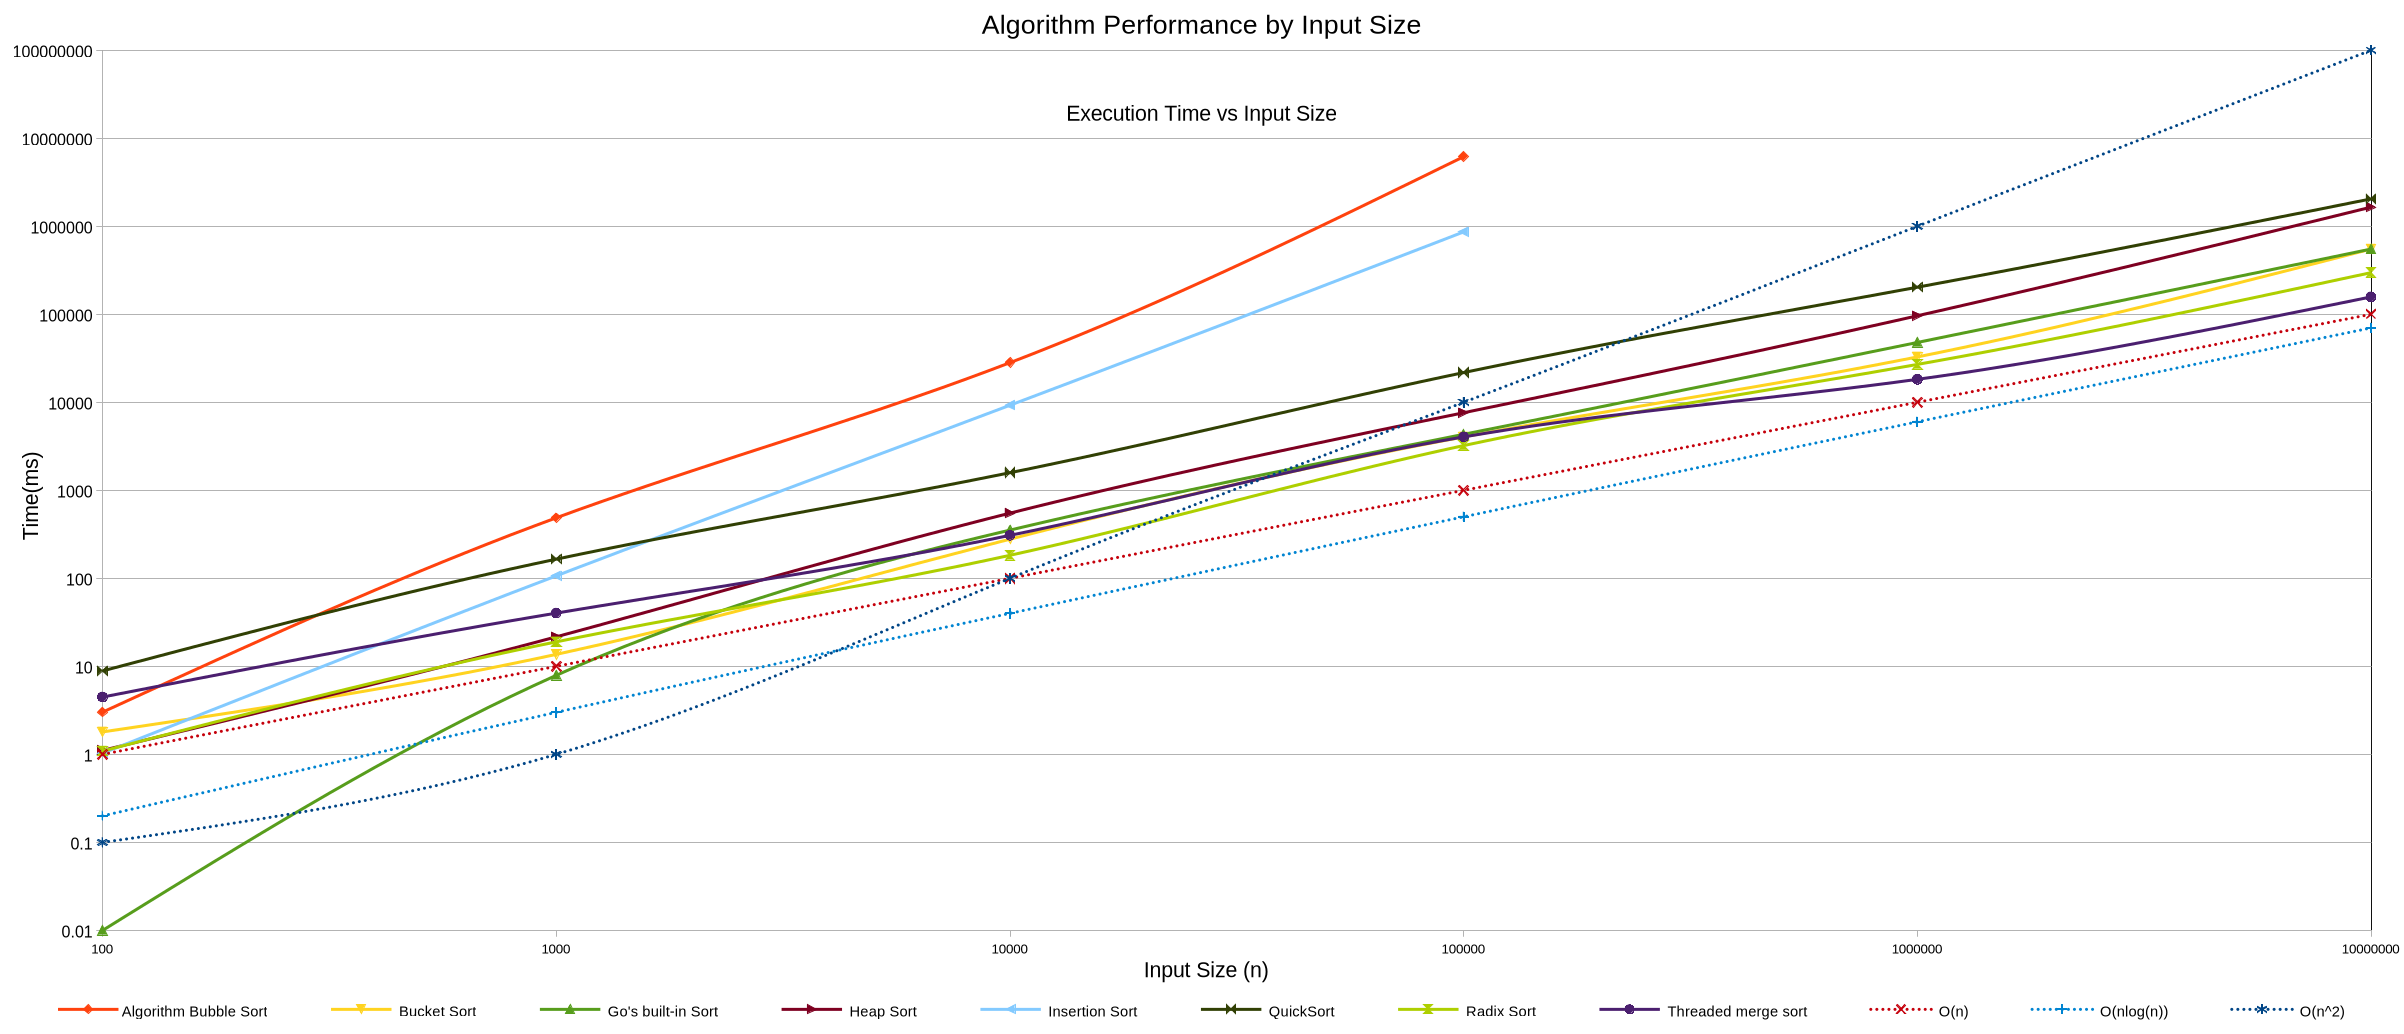
\includegraphics[width=0.8\textwidth]{chart.png}
		\caption{Sorting algorithm benchmark times (ms) by input size, represented as a line chart}
	\end{center}
\end{figure}

\section{Analysis and Conclusions}
The benchmark outcome clearly shows the large difference in performance of the
various sorting algorithms for different input sizes. As predicted,
straightforward quadratic algorithms like Bubble Sort and Insertion Sort have
bad scalability, with running times increasing quickly as the size of the input
increases. For example, Bubble Sort's time leaps from a few milliseconds on
small inputs to several million milliseconds for bigger arrays, making it
impractical for large data sets. On the other hand, algorithms with better
asymptotic complexities, such as

QuickSort, Go native sort (introsort), Heap Sort, and Threaded Merge Sort,
exhibit considerably better performance and scalability. QuickSort tends to be
consistently fast due to its average-case \(O(n \log n)\) complexity, while the
Go native sort utilizes very optimized introsort, leading to the lowest
execution times in most scenarios. Radix Sort and Bucket Sort, that utilize
non-comparison based sorting

methods, execute competitively especially on large sets of data, capitalizing
on their linear or near-linear time complexities under optimal conditions. The
results also confirm the expected trade-offs between algorithm complexity,
implementation concerns, and parallelism (for Threaded Merge Sort). Exclusion
of Bubble Sort and Insertion Sort for the largest dataset was justified given
their infeasible runtimes. Generally, this evidence corroborates the
theoretical time complexities and affirms the importance of choosing an optimal
sorting algorithm based on dataset size and performance requirements.





\end{document}

